Para generar los lotes de prueba se creó un programa especial capaz de generar instancias aleatorias del problema. Los grafos de prueba se separaron en dos grupos:
\begin{itemize}
 \item 30-densos
 \item 70-densos
\end{itemize}
Esta nomenclatura hace referencia al parámetro \probabilidad{probabilidad} con el que los lotes fueron generados. El generador de casos permite introducir un valor entero \textbf{p} entre 1 y 100 que indica para cada par de nodos, la probabilidad de que éstos se conecten al momento de generarción del lote. Esto nos permitió generar grafos mas densos o menos densos, haciendo referencia a la cantidad de amigas de cada alumna. 
También el programa generador de casos de prueba permite generar casos completamente aleatorios o, una vez generado, ajustarlo para que no sea interceptado por los casos de optimización del algoritmo (teoremas de Dirac y Ore). Esto nos dió la posibilidad de ver el desempeño de la parte del 
algoritmo que mayor aporte hace a la complejidad del problema. Aquellos lotes de este tipo se identifican con la sigla \textbf{NT}, haciendo referencia a que no cumplen las hipótesis de los 
casos de optimización (salvo el caso en que los nodos tienen 0 o 1 vecino).
Por último cabe aclarar que cada lote cuenta con 10 casos para cada n, de los cuales se extrajo el mínimo y el promedio, y que la escala de los gráficos es \textbf{logarítmica} para los tiempos.
\newline
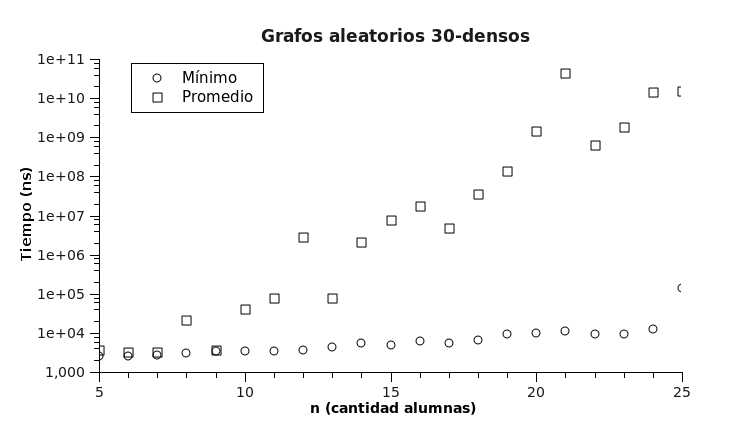
\includegraphics[scale=0.8]{img/ej2/tests/30d_lote1.png}
\newline
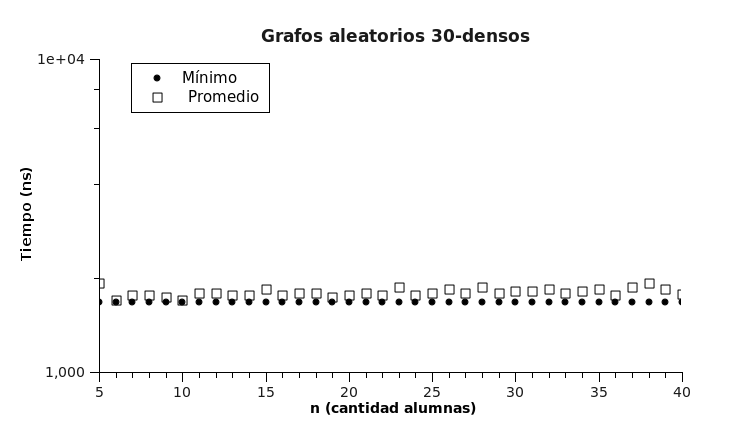
\includegraphics[scale=0.8]{img/ej2/tests/30d_lote2.png}
\newline
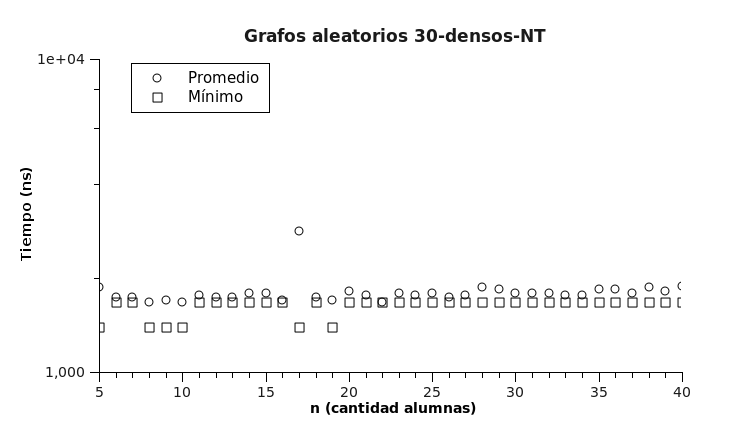
\includegraphics[scale=0.8]{img/ej2/tests/30d_nt_lote1.png}
\newline
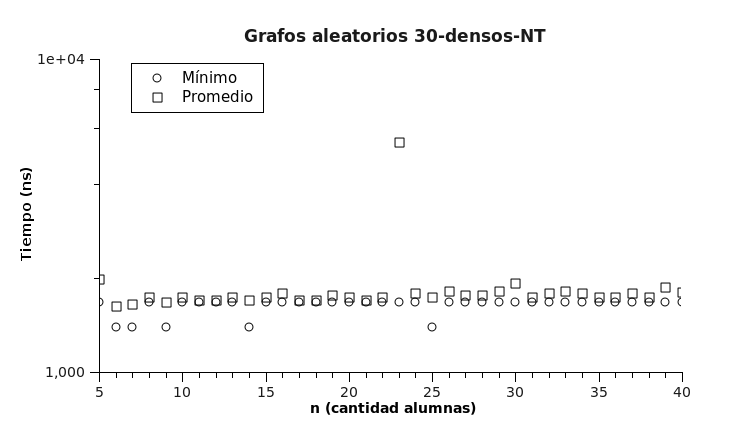
\includegraphics[scale=0.8]{img/ej2/tests/30d_nt_lote2.png}
\newline
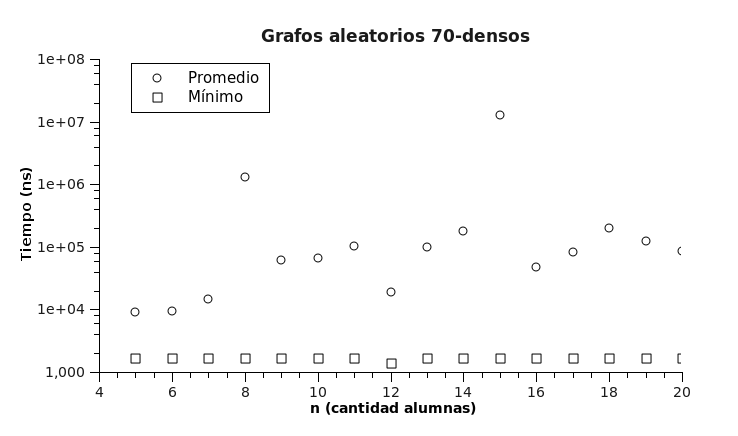
\includegraphics[scale=0.8]{img/ej2/tests/70d_lote1.png}
\newline
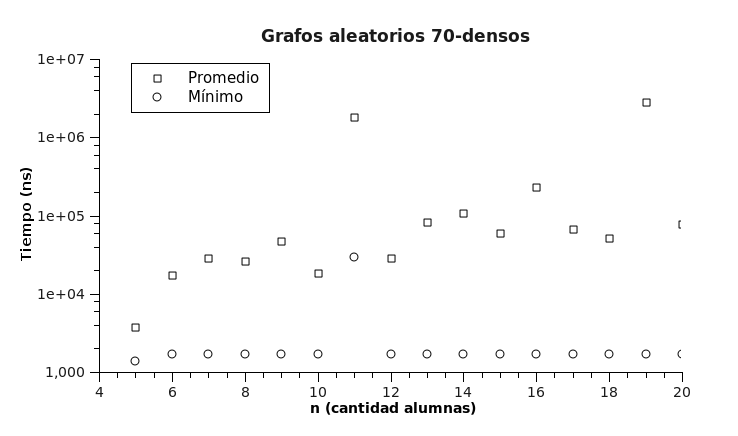
\includegraphics[scale=0.8]{img/ej2/tests/70d_lote2.png}
\newline
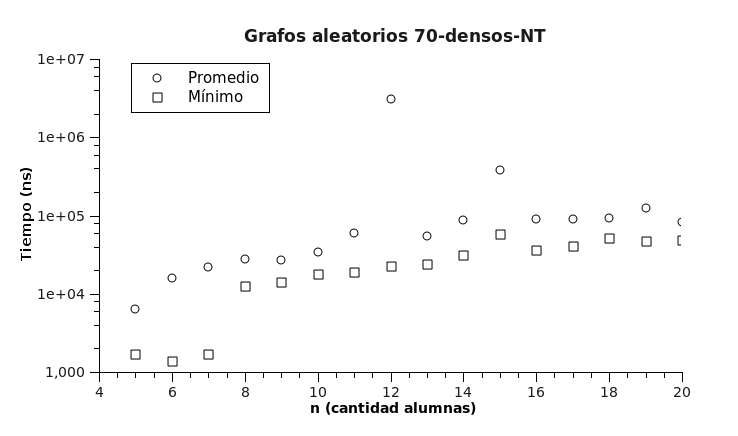
\includegraphics[scale=0.8]{img/ej2/tests/70d_nt_lote1.png}
\newline
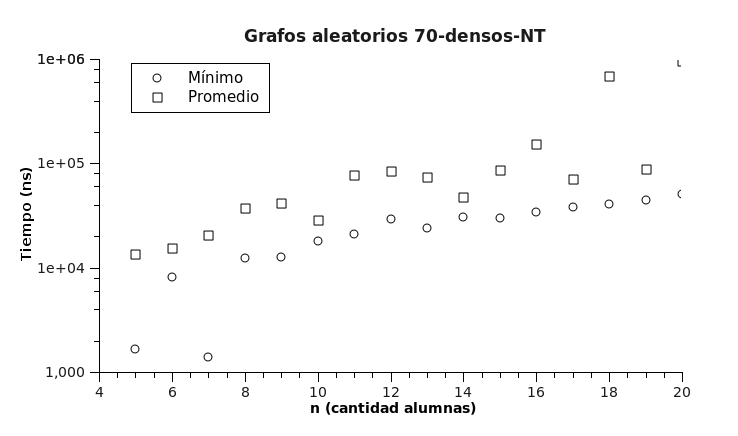
\includegraphics[scale=0.8]{img/ej2/tests/70d_nt_lote2.png}
\newline

En cuanto al peor caso, no pudimos obtener una forma general para el mismo y por lo tanto un algoritmo que lo generase. Aún cuando hubieramos podido armar dichos casos, la naturaleza 
del problema, y sobre todo nuestro algoritmo hace que los tiempos de casos malos se disparen, tardando incluso varias decenas de minutos para casos grandes. Es por eso que no se incluyen tests 
del peor caso.